\ifx\wholebook\relax \else
% ------------------------

\documentclass[UTF8]{article}
%------------------- Other types of document example ------------------------
%
%\documentclass[twocolumn]{IEEEtran-new}
%\documentclass[12pt,twoside,draft]{IEEEtran}
%\documentstyle[9pt,twocolumn,technote,twoside]{IEEEtran}
%
%-----------------------------------------------------------------------------
\input{../../../common-en.tex}

\setcounter{page}{1}

\begin{document}

%--------------------------

% ================================================================
%                 COVER PAGE
% ================================================================

\title{AVL tree - proofs and deletion algorithm}

\author{Larry~LIU~Xinyu
\thanks{{\bfseries Larry LIU} \newline
  Email: liuxinyu95@gmail.com \newline}
  }

\maketitle
\fi

\markboth{AVL tree - proofs and deletion algorithm}{Elementary Algorithms}

\ifx\wholebook\relax
\chapter{AVL tree - proofs and deletion algorithm}
\numberwithin{Exercise}{chapter}
\fi

% ================================================================
%                 Introduction
% ================================================================

This appendix provides proofs to result we uses in the AVL tree pattern
matching insert algorithm.

\section{Height increment after insertion}

When insert a key to the AVL tree, the increment to the height can be deduced
into four cases given as below.

\[
\begin{array}{rl}
  \Delta H & = |T'| - |T| \\
              & = \left \{
                  \begin{array}{r@{\quad:\quad}l}
                  \Delta H_r & \Delta \geq 0 \land \Delta' \geq 0 \\
                  \Delta + \Delta H_r & \Delta \leq 0 \land \Delta' \geq 0 \\
                  \Delta H_l - \Delta & \Delta \geq 0 \land \Delta' \leq 0 \\
                  \Delta H_l & otherwise
                  \end{array} \right .
\end{array}
\]

To prove this equation, note the fact that the height can't increase
both in left and right with only one insertion.

These 4 cases can be explained from the balance factor
definition that it equals to the difference of the right and left sub trees.

\begin{itemize}
\item If $\Delta \geq 0$ and $\Delta' \geq 0$, it means that the height
of right sub tree isn't less than the left sub tree
before and after insertion. In this case, the increment in
height of the tree only is `contributed' from the right sub tree, which
is $\Delta H_r$.

\item If $\Delta \leq 0$, it means the height of left sub tree isn't
less than the right before. Since $\Delta' \geq 0$ after insertion,
we know the height of right sub tree increases,
and the left side keeps same ($|T_l'|=|T_l|$). The increment in height is
as the following.

\[
\begin{array}{rll}
\Delta H & = max(|T_r'|, |T_l'|) - max (|T_r|, |T_l|) & \{\Delta \leq 0 \land \Delta' \geq 0 \}\\
         & = |T_r'|-|T_l| & \{|T_l|=|T_l'| \}\\
         & = |T_r|+\Delta H_r - |T_l| & \\
         & = \Delta + \Delta H_r &
\end{array}
\]

\item For the case $\Delta \geq 0$ and $\Delta' \leq 0$, similar as the
above one, we can get the below result.

\[
\begin{array}{rll}
\Delta H & = max(|T_r'|, |T_l'|) - max (|T_r|, |T_l|) & \{\Delta \geq 0 \land \Delta' \leq 0 \}\\
         & = |T_l'|-|T_r| & \\
         & = |T_l|+\Delta H_l - |T_r| & \\
         & = \Delta H_l - \Delta&
\end{array}
\]

\item For the last case, both $\Delta$ and $\Delta'$ are no bigger than
zero. It means the height of left sub tree is always greater than or equal
 to the right. The increment in height is only `contributed'
from the left sub tree, which is $\Delta H_l$.
\end{itemize}


\section{Proof to the balance adjustment after insertion}

Given the 4 cases need fix as shown in figure \ref{fig:avl-insert-fix}, The balance factors are either -2, or +2. After adjustment, the factor resumes
to 0. The left and right sub trees have the same height.

\begin{figure}[htbp]
   \begin{center}
     \setlength{\unitlength}{1cm}
     \begin{picture}(15, 15)
        % arrows
        \put(4.5, 9.5){\vector(1, -1){1}}
        \put(4.5, 5){\vector(1, 1){1}}
        \put(10, 9.5){\vector(-1, -1){1}}
        \put(10, 5){\vector(-1, 1){1}}
        % delta values
        \put(5, 13){$\delta(z) = -2$}
        \put(2.5, 12){$\delta(y) = -1$}
        \put(10, 13){$\delta(x) = 2$}
        \put(11.5, 11.5){$\delta(y) = 1$}
        \put(1.5, 5.5){$\delta(z) = -2$}
        \put(3.5, 4){$\delta(x) = 1$}
        \put(12, 5.5){$\delta(x) = 2$}
        \put(10.5, 4){$\delta(z) = -1$}
        \put(7.5, 10){$\delta'(y) = 0$}
        % graphics
	\put(0, 7){\includegraphics[scale=0.5]{../../../datastruct/tree/AVL-tree/img/avl-insert-ll.ps}}
        \put(0, 0){\includegraphics[scale=0.5]{../../../datastruct/tree/AVL-tree/img/avl-insert-lr.ps}}
        \put(7, 7){\includegraphics[scale=0.5]{../../../datastruct/tree/AVL-tree/img/avl-insert-rr.ps}}
        \put(8.5, 0){\includegraphics[scale=0.5]{../../../datastruct/tree/AVL-tree/img/avl-insert-rl.ps}}
        \put(2, 5){\includegraphics[scale=0.5]{../../../datastruct/tree/AVL-tree/img/avl-insert-fixed.ps}}
      \end{picture}
     \caption{4 cases for balancing a AVL tree after insertion} \label{fig:avl-insert-fix-appendix}
  \end{center}
\end{figure}

These four cases are left-left lean, right-right lean, right-left lean,
and left-right lean cases. We denote
the balancing factor before fixing as $\delta(x), \delta(y)$, and $\delta(z)$, while after fixing, they changes to $\delta'(x), \delta'(y)$, and
$\delta'(z)$ respectively.

We'll next prove that, after fixing, we have $\delta(y)=0$ for all
four cases, and we'll provide the result values of $\delta'(x)$ and
$\delta'(z)$.

\subsubsection*{Left-left lean case}

As the structure of sub tree $x$ doesn't change due to fixing, we immediately get
$\delta'(x) = \delta(x)$.

Since $\delta(y) = -1$ and $\delta(z) = -2$, we have

\be
  \begin{array}{l}
  \delta(y) = |C| - |x| = -1 \Rightarrow |C| = |x| - 1 \\
  \delta(z) = |D| - |y| = -2 \Rightarrow |D| = |y| - 2
  \end{array}
  \label{eq:ll-cd}
\ee

After fixing.

\be
  \begin{array}{rll}
  \delta'(z) & = |D| - |C| & \{ From (\ref{eq:ll-cd}) \}\\
             & = |y| - 2 - (|x| - 1) & \\
             & = |y| - |x| - 1 & \{  x \text{ is child of } y \Rightarrow |y|-|x| = 1\} \\
             & = 0 &
  \end{array}
  \label{eq:ll-delta-z}
\ee

For $\delta'(y)$, we have the following fact after fixing.

\be
  \begin{array}{rll}
  \delta'(y) & = |z| - |x| & \\
             & = 1 + max(|C|, |D|) - |x| & \{ \text{By (\ref{eq:ll-delta-z}), we have} |C| = |D|\} \\
             & = 1 + |C| - |x| & \{ \text{By (\ref{eq:ll-cd})}\} \\
             & = 1 + |x| - 1 - |x| & \\
             & = 0 &
  \end{array}
\ee

Summarize the above results, the left-left lean case adjust the balancing
factors as the following.

\be
  \begin{array}{l}
  \delta'(x) = \delta(x) \\
  \delta'(y) = 0 \\
  \delta'(z) = 0
  \end{array}
\ee

\subsubsection*{Right-right lean case}

Since right-right case is symmetric to left-left case, we can easily achieve the result balancing factors as

\be
  \begin{array}{l}
  \delta'(x) = 0 \\
  \delta'(y) = 0 \\
  \delta'(z) = \delta(z)
  \end{array}
  \label{eq:rr-result}
\ee

\subsubsection*{Right-left lean case}

First let's consider $\delta'(x)$. After balance fixing, we have.

\be
  \delta'(x) = |B| - |A|
  \label{eq:rl-dx}
\ee

Before fixing, if we calculate the height of $z$, we can get.

\be
  \begin{array}{rll}
  |z| & = 1 + max(|y|, |D|) &  \{ \delta(z) = -1 \Rightarrow |y| > |D|\} \\
      & = 1 + |y| & \\
      & = 2 + max(|B|, |C|)
  \end{array}
  \label{eq:rl-z}
\ee

While since $\delta(x) = 2$, we can deduce that.

\be
  \begin{array}{rll}
  \delta(x) = 2 & \Rightarrow |z| - |A| = 2 & \{ \text{By (\ref{eq:rl-z})} \}\\
                & \Rightarrow 2 + max(|B|, |C|) - |A| = 2 & \\
                & \Rightarrow max(|B|, |C|) - |A| = 0 &
  \end{array}
  \label{eq:rl-ca}
\ee

If $\delta(y) = 1$, which means $|C| - |B| = 1$, it means

\be
  max(|B|, |C|)= |C| = |B|+1
\ee

Take this into (\ref{eq:rl-ca}) yields

\be
  \begin{array}{ll}
  |B|+1-|A| = 0 \Rightarrow |B|-|A|= -1 & \{ \text{By (\ref{eq:rl-dx}) } \} \\
  \Rightarrow \delta'(x) = -1 &
  \end{array}
\ee

If $\delta(y) \neq 1$, it means $max(|B|, |C|) = |B|$, taking this into
(\ref{eq:rl-ca}), yields.

\be
  \begin{array}{ll}
  |B| - |A| = 0  & \{ \text{By (\ref{eq:rl-dx})} \} \\
  \Rightarrow \delta'(x) = 0 &
  \end{array}
\ee

Summarize these 2 cases, we get relationship of $\delta'(x)$ and
$\delta(y)$ as the following.

\be
\delta'(x) = \left \{
  \begin{array}
  {r@{\quad:\quad}l}
  -1 & \delta(y) = 1 \\
  0 & otherwise
  \end{array}
\right.
\label{eq:rl-dx-dy}
\ee

For $\delta'(z)$ according to definition, it is equal to.

\be
  \begin{array}{rll}
    \delta'(z) & = |D| - |C| & \{ \delta(z) = -1 = |D| - |y| \} \\
               & = |y| - |C| - 1 & \{ |y| = 1 + max(|B|, |C|) \} \\
               & = max(|B|, |C|) - |C|
  \end{array}
  \label{eq:rl-dz}
\ee

If $\delta(y) = -1$, then we have $|C| - |B| = -1$, so $max(|B|, |C|) = |B| = |C| + 1$. Takes this into (\ref{eq:rl-dz}), we get $\delta'(z) = 1$.

If $\delta(y) \neq -1$, then $max(|B|, |C|) = |C|$, we get $\delta'(z)=0$.

Combined these two cases, the relationship between $\delta'(z)$ and $\delta(y)$ is as below.

\be
\delta'(z) = \left \{
  \begin{array}
  {r@{\quad:\quad}l}
  1 & \delta(y) = -1 \\
  0 & otherwise
  \end{array}
  \right.
  \label{eq:rl-dz-dy}
\ee

Finally, for $\delta'(y)$, we deduce it like below.

\be
  \begin{array}{rl}
  \delta'(y) & = |z| - |x| \\
             & = max(|C|, |D|) - max(|A|, |B|)
  \end{array}
  \label{eq:rl-dy}
\ee

There are three cases.
\begin{itemize}

\item If $\delta(y)=0$, it means $|B|=|C|$, and according to (\ref{eq:rl-dx-dy}) and (\ref{eq:rl-dz-dy}), we have $\delta'(x)=0 \Rightarrow |A| = |B|$, and $\delta'(z)=0 \Rightarrow |C|=|D|$, these lead to $\delta'(y)=0$.

\item If $\delta(y)=1$, From (\ref{eq:rl-dz-dy}), we have $\delta'(z)=0 \Rightarrow |C| = |D|$.
\[
  \begin{array}{rll}
  \delta'(y) & = max(|C|, |D|) - max(|A|, |B|) & \{|C|=|D|\} \\
             & = |C| - max(|A|, |B|) & \{\text{From (\ref{eq:rl-dx-dy}): $\delta'(x)=-1 \Rightarrow |B|-|A|=-1$} \} \\
             & = |C| - (|B| + 1) & \{ \delta(y) = 1 \Rightarrow |C|-|B|=1\} \\
             & = 0
  \end{array}
\]

\item If $\delta(y)=-1$, From (\ref{eq:rl-dx-dy}), we have $\delta'(x)=0 \Rightarrow |A|=|B|$.
\[
  \begin{array}{rll}
  \delta'(y) & = max(|C|, |D|) - max(|A|, |B|) & \{|A|=|B|\} \\
             & = max(|C|, |D|) - |B| & \{ \text{From (\ref{eq:rl-dz-dy}): $|D|-|C|=1$} \} \\
             & = |C| + 1 - |B| & \{  \delta(y) = -1 \Rightarrow |C|-|B|=-1\} \\
             & = 0
  \end{array}
\]

\end{itemize}

All three cases lead to the same result that $\delta'(y)=0$.

Collect all the above results, we get the new balancing factors after fixing as the following.

\be
  \begin{array}{l}
  \delta'(x) = \left \{
    \begin{array}
    {r@{\quad:\quad}l}
    -1 & \delta(y) = 1 \\
    0 & otherwise
    \end{array}
    \right. \\
  \delta'(y) = 0 \\
  \delta'(z) = \left \{
    \begin{array}
    {r@{\quad:\quad}l}
    1 & \delta(y) = -1 \\
    0 & otherwise
    \end{array}
    \right.
  \end{array}
  \label{eq:rl-result}
\ee

\subsubsection*{Left-right lean case}

Left-right lean case is symmetric to the Right-left lean case. By using
the similar deduction, we can find the new balancing factors are identical
to the result in (\ref{eq:rl-result}).

\section{Deletion algorithm}

Deletion can reduce the height of the sub tree where the node is removed.
If the balance factor exceeds the range of $[-1, 1]$, then we need fix
to resume the AVL properties.

\subsection{Functional deletion}

We can reuse most of the deletion algorithm for BST, then check the balance factor
and perform fixing. Similiar to the insertion algorithm, the result after deletion
is a pair $(T', \Delta H)$, where $T'$ is the new tree and $\Delta H$ is the decrement
of the height. Let function $first(pair)$ return the first component in a pair.
We define the deletion algorithm as below.

\be
delete(T, k) = first(del(T, k))
\ee

where

\be
del(T, k) = \left \{
  \begin{array}
  {r@{\quad:\quad}l}
  (\phi, 0) & T = \phi \\
  tree(del(T_l, k), k', (T_r, 0), \Delta) & k < k' \\
  tree((T_l, 0), k', del(T_r, k), \Delta) & k > k' \\
  (T_r, -1) & k = k', T_l = \phi \\
  (T_l, -1) & k = k', T_r = \phi \\
  tree((T_l, 0), k'', del(T_r, k''), \Delta) & otherwise, k'' = min(T_r)
  \end{array}
\right.
\label{eq:avl-del}
\ee

If the tree is empty, the result is empty as well; Otherwise, we compare the
key with the value to be delete and recursively lookup and perform delete
along the sub trees. If the node to be delete has only one child, we cut
that node off. Otherwise, we use the minimum value in the right sub tree
to replace the key, and cut the minimum node off.

We can reuse the $tree()$ function, as well as the result for $\Delta H$.
But different from insertion, there are extra two cases can violate AVL
properties, thus need fixing.

\begin{figure}[htbp]
  \centering
  \subfloat[Fix AVL violation after deletion. case A]{
    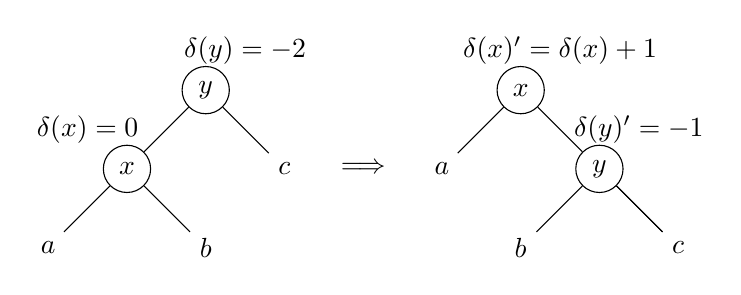
\begin{tikzpicture}[scale=1,
        trnode/.style={circle, draw, inner sep= 0pt, minimum size = .6cm}
      ]
      % left side
      \node[trnode] at (0, 0) (y) {$y$};
      \node[trnode] at (-1, -1) (x) {$x$};
      \draw (1, -1) node (c) {$c$};
      \draw (-2, -2) node (a) {$a$};
      \draw (0, -2) node (b) {$b$};
      % edges
      \draw (y) -- (x) -- (a);
      \draw (y) -- (c);
      \draw (x) -- (b);
      % labels
      \draw (0.5, 0.5) node{$\delta(y) = -2$};
      \draw (-1.5, -0.5) node{$\delta(x) = 0$};

      % right side
      \node[trnode] at (4, 0) (x1) {$x$};
      \draw (3, -1) node (a1) {$a$};
      \node[trnode] at (5, -1) (y1) {$y$};
      \draw (4, -2) node (b1) {$b$};
      \draw (6, -2) node (c1) {$c$};
      % edges
      \draw (x1) -- (y1) -- (c1);
      \draw (x1) -- (a1);
      \draw (y1) -- (b1);
      \draw (y1) -- (c1);
      % labels
      \draw (4.5, 0.5) node{$\delta(x)' = \delta(x) + 1$};
      \draw (5.5, -0.5) node{$\delta(y)' = -1$};

      \draw (2, -1) node{$\Longrightarrow$};
  \end{tikzpicture}} \\
  \subfloat[Fix AVL violation after deletion. case B]{
    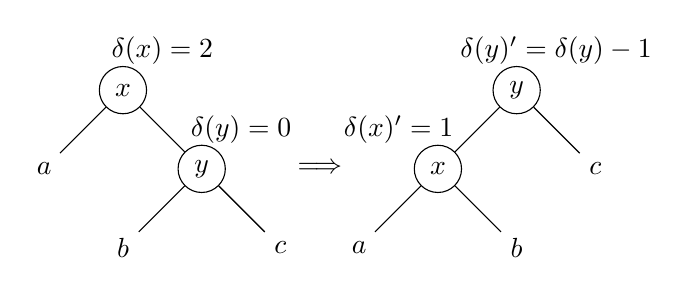
\begin{tikzpicture}[scale=1,
        trnode/.style={circle, draw, inner sep= 0pt, minimum size = .6cm}
      ]
      % left side
      \node[trnode] at (0, 0) (x) {$x$};
      \draw (-1, -1) node (a) {$a$};
      \node[trnode] at (1, -1) (y) {$y$};
      \draw (0, -2) node (b) {$b$};
      \draw (2, -2) node (c) {$c$};
      % edges
      \draw (x) -- (y) -- (c);
      \draw (x) -- (a);
      \draw (y) -- (b);
      \draw (y) -- (c);
      % labels
      \draw (0.5, 0.5) node{$\delta(x) = 2$};
      \draw (1.5, -0.5) node{$\delta(y) = 0$};

      % right side
      \node[trnode] at (5, 0) (y1) {$y$};
      \node[trnode] at (4, -1) (x1) {$x$};
      \draw (6, -1) node (c1) {$c$};
      \draw (3, -2) node (a1) {$a$};
      \draw (5, -2) node (b1) {$b$};
      % edges
      \draw (y1) -- (x1) -- (a1);
      \draw (y1) -- (c1);
      \draw (x1) -- (b1);
      % labels
      \draw (5.5, 0.5) node{$\delta(y)' = \delta(y) - 1$};
      \draw (3.5, -0.5) node{$\delta(x)' = 1$};


      \draw (2.5, -1) node{$\Longrightarrow$};
  \end{tikzpicture}}
  \caption{AVL tree fixing for delete} \label{fig:avl-del-fixing}
\end{figure}

As shown in figure \ref{fig:avl-del-fixing}, both cases can be fixed by a tree rotation. It can be essentailly catpured by pattern matching to the tree structure.

\be
balance(T, \Delta H) = \left \{
  \begin{array}
  {r@{\quad:\quad}l}
  ... \\
  (A, x, (B, y, C, -1), \delta(x) + 1, \Delta H) & T = ((A, x, B \delta(x)), y, C, -2, \Delta H) \\
  ((A, x, B 1), y, C, \delta(y) - 1, \Delta H) & T = (A, x, (B, y, C \delta(y)), 2, \Delta H) \\
  ...
  \end{array}
\right.
\ee

Below is the example program in Haskell

\lstset{language=Haskell}
\begin{lstlisting}
delete::(Ord a) => AVLTree a -> a -> AVLTree a
delete t x = fst $ del t x where
  -- result is a pair (t, d), t: tree, d: decrement in height
  del Empty _ = (Empty, 0)
  del (Br l k r d) x
    | x < k = node (del l x) k (r, 0) d
    | x > k = node (l, 0) k (del r x) d
    -- x == k, delete this node
    | isEmpty l = (r, -1)
    | isEmpty r = (l, -1)
    | otherwise = node (l, 0) k' (del r k') d where k' = min r
\end{lstlisting}

Where the auxiliary function \texttt{min} are implemented similiar to the binary
search tree, it traverses along the left sub tree till the end. Function \texttt{isEmpty} test if a tree is empty.

\begin{lstlisting}
isEmpty Empty = True
isEmpty _ = False

min :: AVLTree a -> a
min (Br Empty x _ _) = x
min (Br l _ _ _) = min l
\end{lstlisting}

After adding the extra two cases for fixing, there are total 7 cases in the \texttt{balance} function.

\begin{lstlisting}
balance :: (AVLTree a, Int) -> (AVLTree a, Int)
balance (Br (Br (Br a x b dx) y c (-1)) z d (-2), dH) =
        (Br (Br a x b dx) y (Br c z d 0) 0, dH-1)
balance (Br a x (Br b y (Br c z d dz)    1)    2, dH) =
        (Br (Br a x b 0) y (Br c z d dz) 0, dH-1)
balance (Br (Br a x (Br b y c dy)    1) z d (-2), dH) =
        (Br (Br a x b dx') y (Br c z d dz') 0, dH-1) where
    dx' = if dy ==  1 then -1 else 0
    dz' = if dy == -1 then  1 else 0
balance (Br a x (Br (Br b y c dy) z d (-1))    2, dH) =
        (Br (Br a x b dx') y (Br c z d dz') 0, dH-1) where
    dx' = if dy ==  1 then -1 else 0
    dz' = if dy == -1 then  1 else 0
-- Delete specific fixing
balance (Br (Br a x b dx) y c (-2), dH) = (Br a x (Br b y c (-1)) (dx+1), dH)
balance (Br a x (Br b y c dy)    2, dH) = (Br (Br a x b    1) y c (dy-1), dH)
balance (t, d) = (t, d)
\end{lstlisting}

\subsection{Imperative deletion}

Imperative deletion algorithm uses tree rotation to resume the balance of the tree.
There are more cases need to handle. We firstly apply the binary search tree deletion
process, then fix the balance if it violates the AVL properties due to the sub tree
height shrink. The main deletion algorithm is given as the following.

\begin{algorithmic}[1]
\Function{Delete}{$T, x$}
  \If{$x = $ NIL}
    \State \Return $T$
  \EndIf
  \State $p \gets$ \Call{Parent}{$x$}
  \If{\Call{Left}{$x$} = NIL}
    \State $y \gets $ \Call{Right}{$x$}
    \State replace $x$ with $y$
  \ElsIf{\Call{Right}{$x$} = NIL}
    \State $y \gets $ \Call{Left}{$x$}
    \State replace $x$ with $y$
  \Else
    \State $z \gets$ \textproc{Min}(\Call{Right}{$x$})
    \State copy key and satellite date from $z$ to $x$
    \State $p \gets$ \Call{Parent}{$z$}
    \State $y \gets$ \Call{Right}{$z$}
    \State replace $z$ with $y$
  \EndIf
  \State \Return \Call{AVL-Delete-Fix}{$T, p, y$}
\EndFunction
\end{algorithmic}

If the node subject to delete is empty, the tree doesn't change. In normal case,
we record the parent of that node as $p$. If either of sub tree is empty, we
cut off the node, and replace it with the other sub tree. Otherwise, we locate
the node contains the minimum key from the right sub tree as $z$, copy the key and the
satellite data to $x$, then cut $z$ off. Finally, we call the fixing function
and pass the root, the parent, and the node replaces the removed one as parameters.

Denote the balance factor of the parent node as $\delta(p)$, by checking the new value
$\delta(p)'$, there are three different cases.

\begin{itemize}
\item Case 1, $|\delta(p)| = 0$, $|\delta(p)'| = 1$. It means, after deletion,
although one sub tree height shrinks, the parent node still satisfies the AVL
property. The algorithm terminates as the tree is still balanced;
\item Case 2, $|\delta(p)| = 1$, $|\delta(p)'| = 0$. It means before the deletion,
the height difference between the two sub trees are 1; while after deletion, the
sub tree with greater height shrinks by 1, thus the heights are same now. As the
result, the height of the parent tree also decrease by 1. We need go on the
botoom-up updating along the parent link towards the root;
\item Case 3, $|\delta(p)| = 1$, $|\delta(p)'| = 2$. It means the tree after deletion
violates the AVL property, we need fix it by tree rotation.
\end{itemize}

For case 3, most of fixing operations are similar to to insertion fixing. However,
we need add two extra sub cases to cover the situations illustrated in figure
\ref{fig:avl-del-fixing}. The fixing algorithm is given as the following.

\begin{algorithmic}[1]
\Function{AVL-Delete-Fix}{$T, p, x$}
  \While{$p \neq $ NIL}
    \State $l \gets$ \Call{Left}{$p$}, $r \gets$ \Call{Right}{$p$}
    \State $\delta \gets \delta(p)$, $\delta' \gets \delta$
    \If{$x = l$}
      \State $\delta' \gets \delta' + 1$
    \Else
      \State $\delta' \gets \delta' - 1$
    \EndIf
    \If{$p$ is leaf} \Comment{$l = r =$ NIL}
      \State $\delta' \gets 0$
    \EndIf
    \If{$|\delta| = 1 \land |\delta'| = 0$}
      \State $x \gets p$
      \State $p \gets$ \Call{Parent}{$x$}
    \ElsIf{$|\delta| = 0 \land |\delta'| = 1$}
      \State \Return $T$
    \ElsIf{$|\delta| = 1 \land |\delta'| = 2$}
      \If{$\delta' = 2$}
        \If{$\delta(r) = 1$} \Comment{Right-right case}
          \State $\delta(p) \gets 0$
          \State $\delta(r) \gets 0$
          \State $p \gets r$
          \State $T \gets $ \Call{Left-Rotate}{$T, p$}
        \ElsIf {$\delta(r) = -1$} \Comment{Right-left case}
          \State $\delta_y \gets \delta($ \Call{Left}{$r$} $)$
          \If{$\delta_y = 1$}
            \State $\delta(p) \gets -1$
          \Else
            \State $\delta(p) \gets 0$
          \EndIf
          \State $\delta($ \Call{Left}{$r$} $) \gets 0$
          \If{$\delta_y = -1$}
            \State $\delta(r) \gets 1$
          \Else
            \State $\delta(r) \gets 0$
          \EndIf
        \Else \Comment{Delete specific right-right case}
          \State $\delta(p) \gets 1$
          \State $\delta(r) \gets \delta(r) - 1$
          \State $T \gets$ \Call{Left-Rotate}{$T, p$}
          \State break \Comment{No furthur height change}
        \EndIf
      \ElsIf{$\delta' = -2$}
        \If{$\delta(l) = -1$} \Comment{Left-left case}
          \State $\delta(p) \gets 0$
          \State $\delta(l) \gets 0$
          \State $p \gets l$
          \State $T \gets $ \Call{Right-Rotate}{$T, p$}
        \ElsIf {$\delta(l) = 1$} \Comment{Left-right case}
          \State $\delta_y \gets \delta($ \Call{Right}{$l$} $)$
          \If{$\delta_y = -1$}
            \State $\delta(p) \gets 1$
          \Else
            \State $\delta(p) \gets 0$
          \EndIf
          \State $\delta($ \Call{Right}{$l$} $) \gets 0$
          \If{$\delta_y = 1$}
            \State $\delta(l) \gets -1$
          \Else
            \State $\delta(l) \gets 0$
          \EndIf
        \Else \Comment{Delete specific left-left case}
          \State $\delta(p) \gets -1$
          \State $\delta(l) \gets \delta(l) + 1$
          \State $T \gets$ \Call{Right-Rotate}{$T, p$}
          \State break \Comment{No furthur height change}
        \EndIf
      \EndIf
      \Comment{Height decrease, go on bottom-up updating}
      \State $x \gets p$
      \State $p \gets$ \Call{Parent}{$x$}
    \EndIf
  \EndWhile
  \If{$p = $ NIL} \Comment{Delete the root}
    \State \Return $x$
  \EndIf
  \State \Return $T$
\EndFunction
\end{algorithmic}

The follow Java example program implements this AVL tree delete algorithm.

\lstset{language=Java}
\begin{lstlisting}
Node del(Node t, Node x) {
    if (x == null) return t;
    Node y, parent = x.parent;
    if (x.left == null) {
        y = x.replaceWith(x.right);
    } else if (x.right == null) {
        y = x.replaceWith(x.left);
    } else {
        y = min(x.right);
        x.key = y.key;
        parent = y.parent;
        y = y.replaceWith(y.right);
    }
    return deleteFix(t, parent, y);
}
\end{lstlisting}

\begin{lstlisting}
Node deleteFix(Node t, Node parent, Node x) {
    while (parent != null) {
        int d1 = parent.delta;
        int d2 = d1 + (x == parent.left ? 1 : -1);
        if (isLeaf(parent))
            d2 = 0;
        parent.delta = d2;
        Node p = parent;
        Node l = parent.left;
        Node r = parent.right;
        if (abs(d1) == 1 && abs(d2) == 0) {
            x = parent;
            parent = x.parent;
        } else if (abs(d1) == 0 && abs(d2) == 1) {
            return t;
        } else if (abs(d1) == 1 && abs(d2) == 2) {
            if (d2 == 2) {
                if (r.delta == 1) { // right-right case
                    p.delta = 0;
                    r.delta = 0;
                    parent = r;
                    t = rotateLeft(t, p);
                } else if (r.delta == -1) { // right-left case
                    int dy = r.left.delta;
                    p.delta = dy == 1 ? -1 : 0;
                    r.left.delta = 0;
                    r.delta = dy == -1 ? 1 : 0;
                    parent = r.left;
                    t = rotateRight(t, r);
                    t = rotateLeft(t, p);
                } else { // del specific right-right case
                    p.delta = 1;
                    r.delta--;
                    t = rotateLeft(t, p);
                    break; // no furthur height change
                }
            } else if (d2 == -2) {
                if (l.delta == -1) { // left-left case
                    p.delta = 0;
                    l.delta = 0;
                    parent = l;
                    t = rotateRight(t, p);
                } else if (l.delta == 1) { // left-right case
                    int dy = l.right.delta;
                    l.delta = dy == 1 ? -1 : 0;
                    l.right.delta = 0;
                    p.delta = dy == -1 ? 1 : 0;
                    parent = l.right;
                    t = rotateLeft(t, l);
                    t = rotateRight(t, p);
                } else { // del specific left-left case
                    p.delta = -1;
                    l.delta++;
                    t = rotateRight(t, p);
                    break; // no further height change
                }
            }
            // the 4 rebalance cases cause height decrease, need bottom-up update
            x = parent;
            parent = x.parent;
        }
    }
    if (parent == null) // delete the root
        return x;
    return t;
}
\end{lstlisting}

\begin{Exercise}
Compare the imperative AVL tree fixing algorithms for insertion and deletion, there are similarities. Develop a common AVL tree fixing algorith can serve for both insertion and deletion.
\end{Exercise}

\ifx\wholebook\relax \else
%% \begin{thebibliography}{99}

%% \bibitem{CLRS}
%% Thomas H. Cormen, Charles E. Leiserson, Ronald L. Rivest and Clifford Stein.
%% ``Introduction to Algorithms, Second Edition''. ISBN:0262032937. The MIT Press. 2001

%% \end{thebibliography}

\end{document}
\fi
